\section{Lec 6}
\subsection{Energy \& momentum}
Since out goal is to get to the Einstein Equation, we know that in there there should be the \emph{energy momentum tensor} $T^{\mu \nu }$. \\
As always we will study everything for a flat space-time but it will be useful for non flat ones. \\
We already saw the four-velocity $u^{\mu}$:
\[
u^{\mu } \equiv \frac{d x^{\mu }}{d\tau }
\]
while the proper time is $\Delta \tau^{2} = - \eta_{\mu \nu }dx^{\mu }dx^{\nu }$. \\
We need to make clear that we are talking about a time-like space-time trajectory, so $\Delta s^{2}<0$. \\
Let's start with the WL of a single particle, this is specified by a map $\mathbb{R}\to M$, where $M$ is a manifold that represents spacetime. We usually think the path as a curve parameterized by $\lambda $ so $x^{\mu }\left( \lambda  \right)$. \\
We also use as parameter the $\tau $ so $x^{\mu }\left( \tau  \right)$, this has some advantages because maybe it could be easier to switch to four-velocity.
\begin{equation}
u^{\mu }u_{\mu } = u_{\mu }u^{\mu } = \eta_{\mu \nu } u^{\mu }u^{\nu } = -1
\end{equation}
By the way, four-velocity is what we need to find the \emph{four momentum}:
\begin{equation}
p^{\mu } \equiv m u^{\mu }
\end{equation}
where m is the rest mass that has the same values $\forall$ RF, and it's just a number.

So in rest frame (x',y',z'):

\noindent
\begin{minipage}[t]{0.48\textwidth}
    \vspace*{0pt}
    

\tikzset{every picture/.style={line width=0.75pt}} %set default line width to 0.75pt        

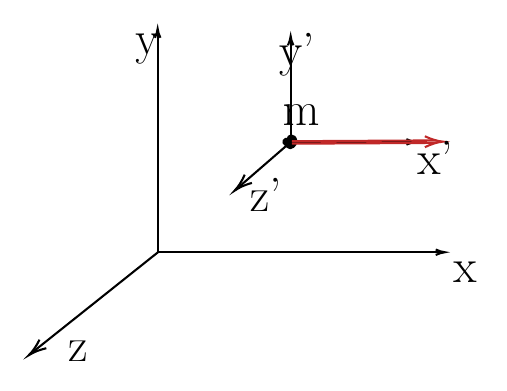
\begin{tikzpicture}[x=0.3pt,y=0.3pt,yscale=-1,xscale=1]
%uncomment if require: \path (0,514); %set diagram left start at 0, and has height of 514

%Straight Lines [id:da944915482116456] 
\draw    (250.32,299.23) -- (250.32,32) ;
\draw [shift={(250.32,30)}, rotate = 90] [color={rgb, 255:red, 0; green, 0; blue, 0 }  ][line width=0.75]    (10.93,-3.29) .. controls (6.95,-1.4) and (3.31,-0.3) .. (0,0) .. controls (3.31,0.3) and (6.95,1.4) .. (10.93,3.29)   ;
%Straight Lines [id:da15966795743012707] 
\draw    (250.32,299.23) -- (594.16,299.23) ;
\draw [shift={(596.16,299.23)}, rotate = 180] [color={rgb, 255:red, 0; green, 0; blue, 0 }  ][line width=0.75]    (10.93,-3.29) .. controls (6.95,-1.4) and (3.31,-0.3) .. (0,0) .. controls (3.31,0.3) and (6.95,1.4) .. (10.93,3.29)   ;
%Straight Lines [id:da1019518678879453] 
\draw    (250.73,299.23) -- (96.56,422.08) ;
\draw [shift={(95,423.32)}, rotate = 321.45] [color={rgb, 255:red, 0; green, 0; blue, 0 }  ][line width=0.75]    (21.86,-6.58) .. controls (13.9,-2.79) and (6.61,-0.6) .. (0,0) .. controls (6.61,0.6) and (13.9,2.79) .. (21.86,6.58)   ;
%Straight Lines [id:da7761915086395399] 
\draw    (410.52,166.36) -- (410.52,41) ;
\draw [shift={(410.52,39)}, rotate = 90] [color={rgb, 255:red, 0; green, 0; blue, 0 }  ][line width=0.75]    (10.93,-3.29) .. controls (6.95,-1.4) and (3.31,-0.3) .. (0,0) .. controls (3.31,0.3) and (6.95,1.4) .. (10.93,3.29)   ;
%Straight Lines [id:da2518341020035201] 
\draw    (410.52,166.36) -- (558.87,166.36) ;
\draw [shift={(560.87,166.36)}, rotate = 180] [color={rgb, 255:red, 0; green, 0; blue, 0 }  ][line width=0.75]    (10.93,-3.29) .. controls (6.95,-1.4) and (3.31,-0.3) .. (0,0) .. controls (3.31,0.3) and (6.95,1.4) .. (10.93,3.29)   ;
%Straight Lines [id:da6843037394854449] 
\draw    (410.7,166.36) -- (344.51,223.76) ;
\draw [shift={(343,225.07)}, rotate = 319.07] [color={rgb, 255:red, 0; green, 0; blue, 0 }  ][line width=0.75]    (21.86,-6.58) .. controls (13.9,-2.79) and (6.61,-0.6) .. (0,0) .. controls (6.61,0.6) and (13.9,2.79) .. (21.86,6.58)   ;
%Shape: Free Drawing [id:dp9557143063465285] 
\draw  [line width=3] [line join = round][line cap = round] (410.85,166.25) .. controls (410.85,167.51) and (410.44,163.59) .. (410.85,162.46) .. controls (411.44,160.78) and (416.94,165.75) .. (410.85,170.04) .. controls (409.05,171.31) and (407.47,166.25) .. (405.46,166.25) ;
%Straight Lines [id:da5108630624179767] 
\draw [color={rgb, 255:red, 192; green, 40; blue, 40 }  ,draw opacity=1 ]   (411.99,165.5) -- (585.99,164.54)(412.01,168.5) -- (586.01,167.54) ;
\draw [shift={(594,166)}, rotate = 179.69] [color={rgb, 255:red, 192; green, 40; blue, 40 }  ,draw opacity=1 ][line width=0.75]    (21.86,-6.58) .. controls (13.9,-2.79) and (6.61,-0.6) .. (0,0) .. controls (6.61,0.6) and (13.9,2.79) .. (21.86,6.58)   ;

% Text Node
\draw (219.7,32.51) node [anchor=north west][inner sep=0.75pt]   [align=left] {{\LARGE y}};
% Text Node
\draw (602.64,306.78) node [anchor=north west][inner sep=0.75pt]   [align=left] {{\LARGE x}};
% Text Node
\draw (138.58,401.86) node [anchor=north west][inner sep=0.75pt]   [align=left] {{\LARGE z}};
% Text Node
\draw (397,118) node [anchor=north west][inner sep=0.75pt]   [align=left] {{\LARGE m}};
% Text Node
\draw (392.97,31.76) node [anchor=north west][inner sep=0.75pt]   [align=left] {{\LARGE y'}};
% Text Node
\draw (559.44,161.51) node [anchor=north west][inner sep=0.75pt]   [align=left] {{\LARGE x'}};
% Text Node
\draw (357.7,206.48) node [anchor=north west][inner sep=0.75pt]   [align=left] {{\LARGE z'}};


\end{tikzpicture}

\end{minipage}
\begin{minipage}[t]{0.48\textwidth}
    \vspace*{0pt}
	So in the rest frame (x',y',z'): \\
   $p^{\mu }= \left( m,0,0,0 \right)$, because the \\four-velocity in the rest frame is \\$u^{\mu }= \left( 1,0,0,0 \right)$.  \\
   What is the expression of $p^{\mu }$ in the (x,y.z) frame?\\
   And what is the fastest way to compute it?		
\end{minipage}\hfill

We can start from the rest frame and use a LT. \\
For a generic four vector we have:
\begin{equation}
\begin{cases}
a^{0'} = \gamma \left( a^{0}- va^{1} \right) \\
a^{1'} = \gamma \left( a^{1}-va^{0} \right)\\
 a^{2'} = a^{2} \\
 a^{3'} = a^{3}
\end{cases}
\end{equation}
Now we find the inverse, we can search the inverse of the matrix or use an inverse LT,
\begin{equation}
\begin{cases}
a^{0} = \gamma \left( a^{0'}+va^{1'} \right) \\
a^{1} = \gamma \left( a^{1'}+va^{0'} \right) \\
a^{2} = a^{2'} \\
a^{3} = a^{3'}
\end{cases}
\end{equation}
So for the four-momentum we have:
\begin{equation}
\begin{cases}
	p^{0} = E = \gamma p^{0'} = \gamma m = \frac{m}{\sqrt{1-v^{2}}} \\
	p^{1} = m \gamma v = \frac{mv}{\sqrt{1-v^{2}}} \\
	p^{2} = 0 \\
	p^{3 }= 0
\end{cases}
\end{equation}
In the NR limit we should be able to recover Newton Mechanics:
\begin{gather*}
E  \approx m + \frac{mv^{2}}{2} + \ldots  \\
p^{1} \approx mv + \ldots 
\end{gather*}
The four-momentum as we got it provides the description of a single particle but often we need to study a lot of particles as a continuum, like a \emph{fluid}, characterized by quantities as density, pressure, entropy, viscosity... \\
A single momentum four-vector field is insufficient to describe the energy and the momentum of a fluid so we go further and define the \emph{energy-momentum tensor}.
\subsection{Energy-Momentum Tensor}
\[
T^{\alpha \beta }
\]
For now it is just a tensor, and we are happy to see that it transform like a tensor:
\[
T^{\alpha ' \beta '} = \Lambda^{\alpha '}_{\alpha }\Lambda^{\beta '}_{\beta }T^{\alpha \beta }
\]
In words, it is defined like "\emph{the flux of four-momentum $p^{\alpha }$ across the surface where $x^{\beta }$ is constant}".

For a system of \emph{N} particles we have: 
\[
p^{\alpha } = \sum_{j=1}^{N}{p^{\alpha }_{j}}	 
\]
where \emph{j} shows the \emph{j-th} particle, not an index to contract.
The \emph{number density, n} for a system of \emph{N} particles is:
\[
n = \sum_{j}^{}{\delta\left( \vec{r}-\vec{r}_{j} \right)}
\]
So we have these components of the energy-momentum tensor:
\begin{gather*}
T^{\alpha 0} = \sum_{j}^{}{p^{\alpha }_{j} \frac{dt}{dt} \delta\left( \vec{r}-\vec{r}_{j} \right)} \\
T^{\alpha i} = \sum_{j}^{}{p^{\alpha }_{j} \frac{dx^{i}_{j}}{dt} \delta\left( \vec{r}-\vec{r}_{j} \right) }
\end{gather*}
 
RECUPERA


So what is a tensor?
It is not obvious, so our goal is to prove that this is actually a tensor by see how it transform under LTs.

First thing we compute:
\[
	\left\frac{ dx^{i}_{j} \right}{dt} = \left\frac{ dx^{i}_{j} \right}{d\tau } \colorbox{yellow}{$ \frac{d\tau }{dt}$} = \frac{dx^{i}_{j}}{d\tau } \colorbox{yellow}{$ \frac{1}{\gamma_{j}}$} 
\]
because
\[
\frac{d\tau ^{2}}{dt^{2}} = \frac{dt^{2}-dx^{2}}{dt^{2}} = 1 - v^{2}_{j} = \frac{1}{\gamma^{2}_{j}}
\]
why is it useful? Because it appears in components
\[
\frac{dx^{i}_{j}}{d\tau } = \left( m^{j} \frac{dx^{i}_{j}}{d\tau } \right) \frac{1}{m_{j}\gamma_{j}} = \frac{p^{i}_{j}}{p^{0}_{j}}		
\]
so i can rewrite the energy-momentum tensor like:
\[
T^{\alpha \beta } = \sum_{j}^{}{\frac{ p^{\alpha }_{j}p^{\beta }_{j}}{p^{0}_{j}}\delta\left( \vec{r}-\vec{r}_{j} \right)}
\]
so if 
\begin{itemize}
	\item $\beta =0 \to p^{\alpha }_{j}$ 
	\item $\beta =1 \to \frac{p^{i}_{j}}{p^{0}_{j}}$
\end{itemize}
If i switch $\alpha $ with $\beta $, I find the same objects, because the tensor is symmetric.
\[
	T^{\left( \alpha \beta  \right)} = T^{\alpha \beta } \text{  ;   } T^{[\alpha \beta }]} = 0
\]
Why is a tensor? If I change frame I can change 



